\startchapter{Evaluation}
\label{chapter:Exp}

The case we used to test this prototype contains one named pipe synchronous channel between a server and a client. Client send a message to the server and server reply another message to the client. 
\subsection{Experiment Verification Design}
The test cases are designed to find all the messages from client to server and all the messages from server to client. Two end to end test cases are designed for both scenarios. 

In each test case, there are three test steps: 1. define the communication type by adding channel creating functions and message send/receive functions of server and client sides. 2. search for the events of  the defined communication type. 3. for the occurrence of the events, navigate to the trace instruction and memory view.

Verification points are specified for each step as: 1. verify the communication types with their functions are listed in the communication view. 2. verify the message events in the dual-trace can be found and listed in the search result view. 3. verify the navigation from the result entry to the instruction view of sender trace and receiver trace.
\subsection{Result}
We used the dual-trace provided by DRDC and follow the experiment and verification design to conduct this test. Figure\ref{addcomtyperesult} shows that the user defined clientsend and serversend communication types are shown in the communication type view as well as the functions consist of the communication types. Figure\ref{occclientresult} shows the search result of clientsend communication type, while Figure\ref{occclientresult} shows the search result of the serversend communication type. By clicking the Go To Line of Message Sender and Go To Line of Message Receiver action items, instruction view and memory view updated correctly. Figure\ref{send} shows the server was sending out a message: This is an answer. 


\begin{figure}[H]
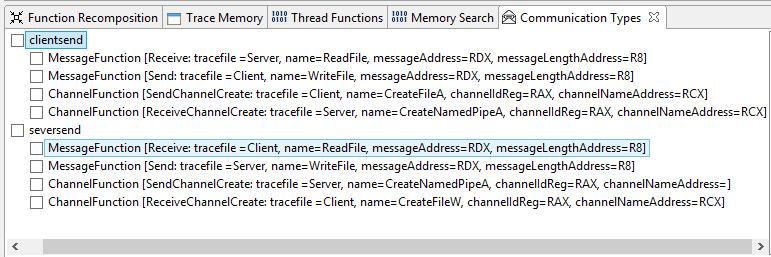
\includegraphics[scale=.72]{Figures/addcomtyperesult}
 \caption{Defined clientsend and serversend communication types in Communication View}
\label{addcomtyperesult}
\end{figure}

\begin{figure}[H]
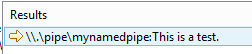
\includegraphics{Figures/occclientresult}
 \caption{the search result of clientsend communication type}
\label{occclientresult}
\end{figure}


\begin{figure}[H]
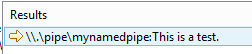
\includegraphics{Figures/occclientresult}
 \caption{the search result of the serversend communication type}
\label{occclientresult}
\end{figure}

\begin{figure}[H]
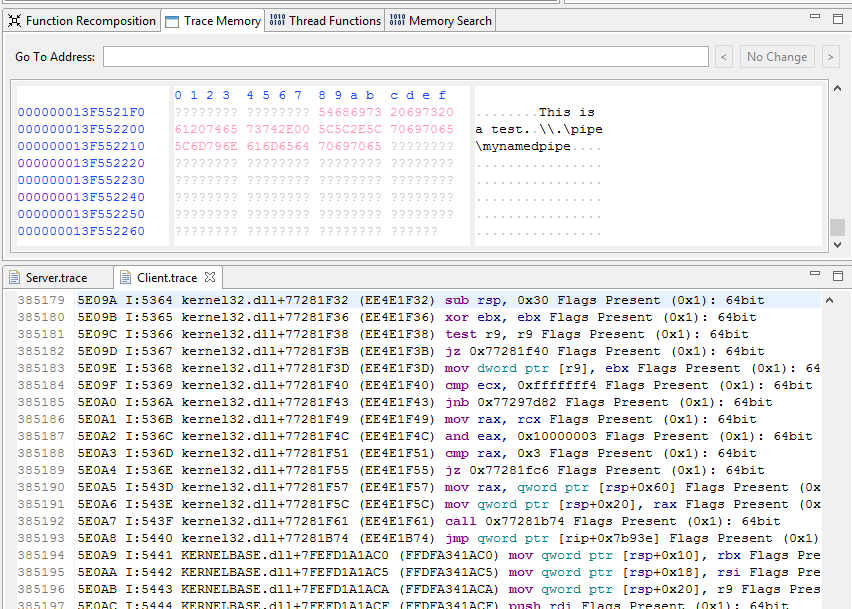
\includegraphics[scale=.66]{Figures/send}
 \caption{instruction view and memory view updated correctly}
\label{send}
\end{figure}
